\documentclass{beamer}

% \usepackage{concmath} 
\usetheme{Boadilla}
\usepackage[utf8]{inputenc}
\usepackage{helvet}
\usepackage[english]{babel}

\usepackage{natbib} % for the bibliography
\setcitestyle{numbers}

\usecolortheme{tum}
\useoutertheme{tum}

\setbeamerfont{author}{size=\footnotesize}
\setbeamerfont{date}{size=\scriptsize}
\setbeamerfont{date}{size=\scriptsize}

\useinnertheme{rectangles}

\usepackage{pgf}  
\usepackage{tikz}
\logo{\pgfputat{\pgfxy(-0.2, 8.5)}{\pgfbox[right,top]{
\begin{tikzpicture}[y=0.38pt, x=0.38pt,yscale=-1, inner sep=0pt, outer sep=0pt]
\begin{scope}[cm={{1.25,0.0,0.0,-1.25,(0.0,35.4325)}}]
    \path[fill=tum,nonzero rule] (4.8090,23.2950) -- (4.8090,-0.0020) --
      (9.8590,-0.0020) -- (9.8590,23.2600) -- (15.4730,23.2600) -- (15.4730,-0.0020)
      -- (31.5390,-0.0020) -- (31.5390,23.0140) -- (37.2580,23.0140) --
      (37.2580,0.0060) -- (42.5550,0.0060) -- (42.5550,23.0140) -- (48.3440,23.0140)
      -- (48.3440,0.0060) -- (53.6410,0.0060) -- (53.6410,28.3460) --
      (26.4530,28.3460) -- (26.4530,5.1580) -- (20.6290,5.1580) -- (20.6290,28.3110)
      -- (-0.0000,28.3110) -- (-0.0000,23.2950) -- (4.8090,23.2950) -- cycle;
\end{scope}
\end{tikzpicture}
}}}

\setbeamertemplate{title page}
{
	\vbox{}
	\vfill
	\begin{flushleft}
		\begin{beamercolorbox}[sep=8pt,left]{title}
			\usebeamerfont{title}\inserttitle\par%
			\ifx\insertsubtitle\@empty%
			\else%
				\vskip0.25em%
				{\usebeamerfont{subtitle}\usebeamercolor[fg]{subtitle}\insertsubtitle\par}%
			\fi%
    	\end{beamercolorbox}%
    	\vskip1em\par
		\begin{beamercolorbox}[sep=8pt,left]{author}
		\usebeamerfont{author}\insertauthor
		\end{beamercolorbox}
		\begin{beamercolorbox}[sep=8pt,left]{institute}
		\usebeamerfont{institute}\insertinstitute
		\end{beamercolorbox}
		\begin{beamercolorbox}[sep=8pt,left]{date}
		\usebeamerfont{date}\insertdate
		\end{beamercolorbox}\vskip0.5em
		{\usebeamercolor[fg]{titlegraphic}\inserttitlegraphic\par}
	\end{flushleft}
	\vfill
}

\mode<presentation>

\title{Source Terms}
% \subtitle{Source Terms}

\author{Matilde Tozzi}
\institute[]{Seminar Course - Fundamentals of Wave Simulation - Solving Hyperbolic Systems of PDEs}
\date[January 2024]{January 2024}

\newcommand{\ca}{\mathcal{A}}
\newcommand{\cb}{\mathcal{B}}
\renewcommand{\d}{\Delta}
\renewcommand{\emph}[1]{\textcolor{tum}{\textbf{#1}}}
\graphicspath{{../Code/}{..}}

\begin{document}
\beamertemplatenavigationsymbolsempty

\begin{frame}
	\titlepage
\end{frame}

% 2. Slide: TOC
\begin{frame}
	\frametitle{Table of contents}
	\tableofcontents
\end{frame}


%%%%%%%%%%%%%%%%%%% From Conservation Laws to Balance Laws
\section{From Conservation Laws to Balance Laws}
\begin{frame}
	\frametitle{From Conservation Laws to Balance Laws}
	Our reference equation is
	\begin{equation}
		q_t +f(q)_x = \psi(q)
	\end{equation}
	where
	\begin{itemize}
		\item the homogeneous equation $q_t +f(q)_x = 0$ is \emph{hyperbolic}
		\item $\psi(q)$ (the \emph{source terms}) don't depend on derivatives of $q$
		      \begin{itemize}
			      \item $\Rightarrow$ $q_t = \psi(q)$ is an independent system of ODEs
		      \end{itemize}
	\end{itemize}
\end{frame}

%%%%%%%%%%%%%%%%%%% Godunov-Strang splitting
\section{Godunov-Strang splitting}

%%%%%%%%%%%%%%%%%%% The Advection-Reaction Equation
\subsection{The Advection-Reaction Equation}

\begin{frame}
	\frametitle{The Advection-Reaction Equation}

	A standard example that will be used to illustrate the following numerical methods is the \emph{advection-reaction equation}

	\begin{equation}\label{eq:advec}
		q_t + \bar{u}q_x=-\beta q.
	\end{equation}

	It can be seen as the model for the transport along a flow of a radioactive substance, where

	\begin{itemize}
		\item $\beta$ is the \emph{decay rate}
		\item $\bar{u}$ is the (constant) \emph{transport speed}
		\item $q(x,0)= \mathring{q}(x)$ is the \emph{initial condition}.
	\end{itemize}
	\pause
	\begin{block}{Exact solution}
		Along the characteristic $\frac{dx}{dt}=\bar{u}$ we have $\frac{dq}{dt}=-\beta q$ and it follows that

		\begin{equation}\label{eq:advec_sol}
			q(x,t) = e^{-\beta t}\mathring{q}(x-\bar{u}t).
		\end{equation}
	\end{block}

\end{frame}

\begin{frame}
	\frametitle{The Advection-Reaction Equation: Plot}
	\begin{figure}[!ht]
		\centering
		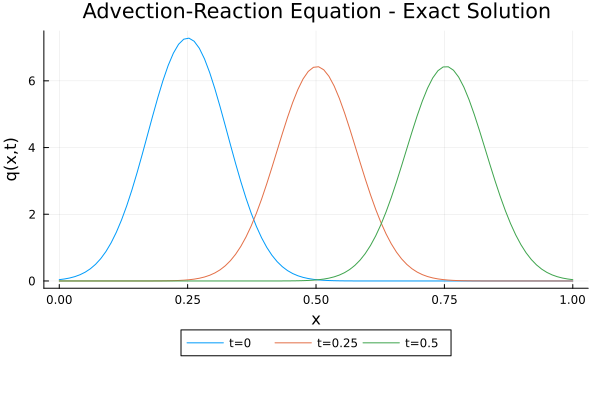
\includegraphics[width=.7\textwidth]{../Advection.png}

		\caption{Evolution of the exact solution of the advection-reaction equation with $\bar{u}=1$, $\beta=1$, and $\mathring{q}=\text{Gaussian}(0.25,0.003)$.}
		\label{fig:exact}
	\end{figure}
\end{frame}

%%%%%%%%%%%%%%%%%%% The Unsplit Method
\subsection{The Unsplit Method}

\begin{frame}
	\frametitle{The Unsplit Method}
	Dor this specific example we can easily compute an \emph{unsplit method}

	\begin{align*}\label{eq:unsplit}
		q_t                          & = -\bar{u}q_x-\beta q                                              \\
		\frac{Q^{n+1}_i-Q^n_i}{\d t} & = -\bar{u} \frac{Q^n_i-Q^n_{i-1}}{\d x}-\beta Q^n_i                \\
		Q^{n+1}_i                    & = Q^n_i-\bar{u} \frac{\d t}{\d x}(Q^n_i-Q^n_{i-1})-\d t\beta Q^n_i
	\end{align*}

	which is first-order accurate and stable for $0<\bar{u}\frac{\d t}{\d x}\leq1$.
\end{frame}

\begin{frame}
	\frametitle{Taylor Expansion of the Exact Solution}
	\begin{block}{Note}
		The full Taylor expansion of \eqref{eq:advec} can be written formally as

		\begin{equation}\label{eq:sol_op}
			\begin{gathered}
				e^{-\d t(\bar{u}\partial_x+\beta)}q(x,t):=q(x,t+\d t)=\\
				=\sum_{j=0}^{\infty}\frac{(\d t)^j}{j!}\partial_t^jq(x,t)=\sum_{j=0}^{\infty}\frac{(\d t)^j}{j!}(-\bar{u}\partial_x-\beta)^jq(x,t).
			\end{gathered}
		\end{equation}

		The operator $e^{-\d t(\bar{u}\partial_x+\beta)}$ is called \emph{solution operator} for the equation \eqref{eq:advec} over a time step of length $\d t$.
	\end{block}
\end{frame}












%%%%%%%%%%%%%%%%%%% Godunov Splitting
\subsection{Godunov Splitting}

\begin{frame}
	\frametitle{Godunov Splitting}
	In the case of the advection equation, we can split it into two subproblems:

	\begin{equation}\label{eq:probA}
		\text{Problem A: } q_t+\bar{u}q_x=0,
	\end{equation}

	\begin{equation}\label{eq:probB}
		\text{Problem B: } q_t = -\beta q.
	\end{equation}

	The idea is to apply the two methods in an alternating manner, using standard solving stategies, e.g.:

	\begin{equation}\label{eq:stepA}
		\text{A-step: } Q_i^* = Q_i^n - \frac{\bar{u}\d t}{\d x} (Q_i^n-Q_{i-1}^n),
	\end{equation}

	\begin{equation}\label{eq:stepB}
		\text{B-step: } Q_i^{n+1} = Q_i^*-\beta\d tQ_i^*.
	\end{equation}

\end{frame}

\begin{frame}
	\frametitle{Unsplit Method vs Godunov Splitting}

	One may think that given that both $Q_i^*$ and $Q_i^{n+1}$ are calculated using $\d t$, the solution is valid for time $2\d t$, but it is not really the case: in fact if we combine the two stages and eliminate $Q_i^*$, we obtain

	\begin{equation*}
		Q_i^{n+1} = Q_i^n -\frac{\bar{u}\d t}{\d x}(Q_i^n-Q_{i-1}^n)-\beta\d tQ_i^n +\frac{\bar{u}\beta\d t^2}{\d x}(Q_i^n-Q_{i-1}^n),
	\end{equation*}

	which differs from the unsplit method for the last term:

	\begin{equation*}
		Q^{n+1}_i = Q^n_i-\bar{u} \frac{\d t}{\d x}(Q^n_i-Q^n_{i-1})-\d t\beta Q^n_i
	\end{equation*}

\end{frame}

\begin{frame}
	\frametitle{Commuting vs Non-commuting operators}
	\begin{figure}[!ht]
		\centering
		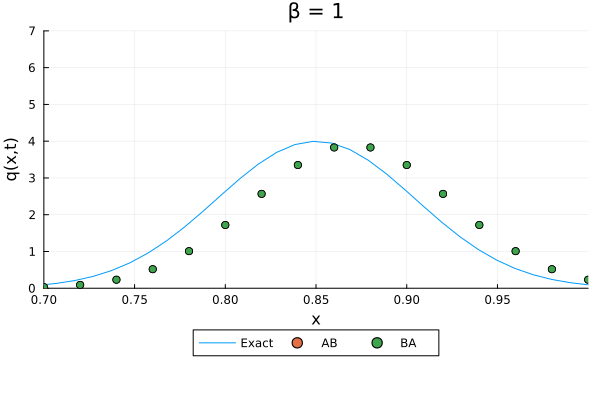
\includegraphics[width=0.4\textwidth]{Commute.png}%
		\label{fig:commute}
		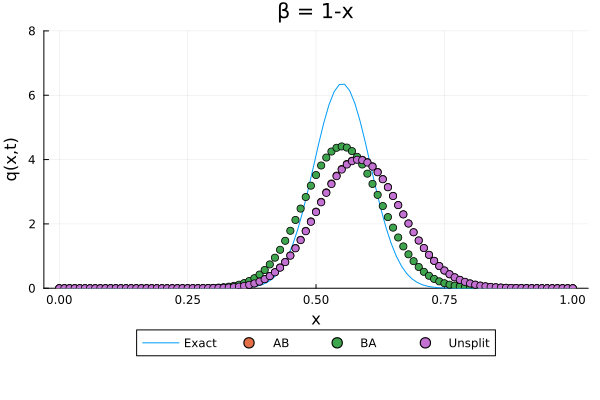
\includegraphics[width=0.4\textwidth]{NoCommute.png}%
		\label{fig:nocommute}

		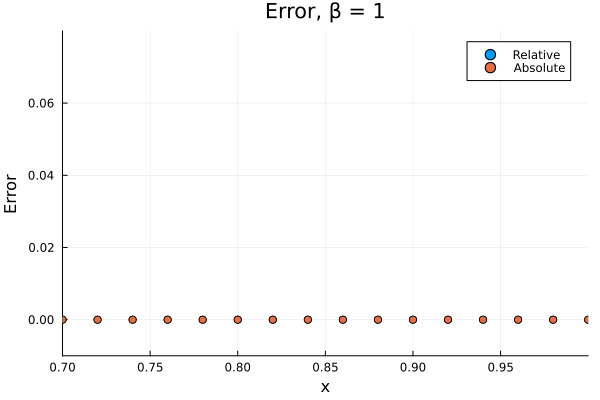
\includegraphics[width=0.4\textwidth]{CommuteErr.png}%
		\label{fig:commuteErr}
		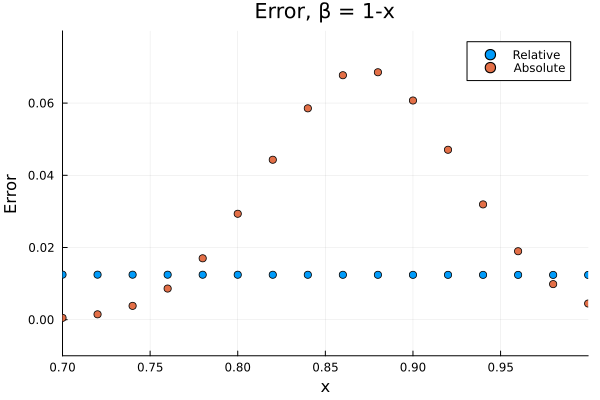
\includegraphics[width=0.4\textwidth]{NoCommuteErr.png}%
		\label{fig:nocommuteErr}
		\caption{Comparison between the exact solution of the advection-reaction equation and the split method with the two different orders of steps. The problem has $\bar{u}=1$, $\mathring{q}=\text{Gaussian}(0.25,0.003)$, $\d x = \d t = 0.02$, $t=0.6$.}
		\label{fi:AB}
	\end{figure}

\end{frame}








%%%%%%%%%%%%%%%%%%% General Formulation
\subsection{General Formulation}
\begin{frame}
	\frametitle{General Formulation}
	Consider the more general formulation

	\begin{equation}
		q_t = (\ca+\cb)q
	\end{equation}

	where $\ca$ and $\cb$ can be differential operators. We assume that they don't explicitly depend on $t$, so that we can write

	\begin{equation}
		q_{tt} = (\ca+\cb)q_t=(\ca+\cb)^2q
	\end{equation}

	If we Taylor expand the solution at time $t$ and use the notation defined in \eqref{eq:sol_op}, we easily get to

	\begin{equation}\label{eq:exp_unsplit}
		q(x,\d t) = \sum_{j=0}^{\infty}\frac{\d t^j}{j!}(\ca + \cb)^jq(x,0) = e^{\d t(\ca +\cb)}q(x,0).
	\end{equation}


\end{frame}

\begin{frame}
	\frametitle{General Formulation II}
	With Godunov Splitting, we obtain

	\begin{equation}
		q^*(x,\d t)=e^{\d t \ca}q(x,0)
	\end{equation}

	and

	\begin{equation}
		q^{**}(x,\d t)=e^{\d t \cb}q^*(x,\d t) = e^{\d t \cb}e^{\d t \ca}q(x,0).
	\end{equation}

	The splitting error is then

	\begin{equation}
		q(x,\d t)-q^{**}(x,\d t) = (e^{\d t(\ca +\cb)}-e^{\d t \cb}e^{\d t \ca})q(x,0).
	\end{equation}

	If we Taylor expand $qx^{**}$, we obtain

	\begin{equation}\label{eq:exp_split}
		q^{**}(x,\d t) = (I+\d t(\ca + \cb)+\frac{1}{2}\d t^2(\ca^2+2\cb\ca+\cb^2)+\dots)q(x,0).
	\end{equation}

\end{frame}














%%%%%%%%%%%%%%%%%%% Strang Splitting
\subsection{Strang Splitting}
\begin{frame}
	\frametitle{Strang Splitting}
	With the \textit{Strang splitting} we are approximating $e^{\d t(\ca +\cb)}$ by $e^{\frac{1}{2}\d t\ca}e^{\d t\cb}e^{\frac{1}{2}\d t\ca}$. The Taylor expansion shows in fact that

	\begin{equation}
		e^{\frac{1}{2}\d t\ca}e^{\d t\cb}e^{\frac{1}{2}\d t\ca} = I+\d t(\ca + \cb)+\frac{1}{2}\d t^2(\ca^2+\ca\cb+\cb\ca+\cb^2)+\mathcal{O}(\d t^3).
	\end{equation}

	After $n$ time steps we obtain

	\begin{equation}\label{eq:recursion}
		Q^n = \underbrace{(e^{\frac{1}{2}\d t\ca}e^{\d t\cb}e^{\frac{1}{2}\d t\ca})(e^{\frac{1}{2}\d t\ca}e^{\d t\cb}e^{\frac{1}{2}\d t\ca})\dots(e^{\frac{1}{2}\d t\ca}e^{\d t\cb}e^{\frac{1}{2}\d t\ca})}_{n\text{ times}}Q^0.
	\end{equation}

	Another way of obtaining the same result is by alternating the oder of application of $\ca$ and $\cb$, in each time step, i.e.

	\begin{equation}
		\begin{gathered}
			Q^1 = e^{\d t\ca}e^{\d t\cb}Q^0\\
			Q^2 = e^{\d t\cb}e^{\d t\ca}Q^1\\
			\vdots
		\end{gathered}
	\end{equation}

	Analogously to our analysis of \eqref{eq:recursion}, we can see that the result is essentially the same, but with $\d t$ instead of $\frac{1}{2}\d t$. This is computationally better because it requires fewer function evaluations, but it is more difficult to implement with variable time steps. Furthermore, it needs an even number of iterations in order to obtain the desired cancellation of errors.
\end{frame}




















%%%%%%%%%%%%%%%%%%% Accuracy
\subsection{Accuracy}
















%%%%%%%%%%%%%%%%%%% Implicit Methods and Choice of ODE Solver
\section{Implicit Methods and Choice of ODE Solver}















%%%%%%%%%%%%%%%%%%% Stiff and Singular Source Terms and the Associated Numerical Difficulties
\section{Stiff and Singular Source Terms and the Associated Numerical Difficulties}




















%%%%%%%%%%%%%%%%%%% Bibliography
\begin{frame}
	\frametitle{Bibliography}
	\bibliographystyle{amsalpha}
	\begin{thebibliography}{1}

		\bibitem{leveque}
		R.~J.~LeVeque, \emph{Finite Volume Methods for Hyperbolic Problems}.\hskip 1em plus
		0.5em minus 0.4em\relax Cambridge: Cambridge University Press, 2002.

		\bibitem{github}
		\url{https://github.com/matilde-t/SeminarCourse-FundamentalsOfWaveSimulation}

		\bibitem{clawpack}
		\url{https://github.com/clawpack/apps/tree/master/fvmbook/chap17}

		\bibitem{riemann}
		\url{https://github.com/clawpack/riemann_book}

	\end{thebibliography}
\end{frame}

\end{document}